\chapter{Trabajo Futuro}
\label{chap:futurework}

En este cap�tulo se explica el trabajo que queda pendiente para el futuro.

\section{Aplicaci�n M�vil para iOS}

La idea inicial era desarrollar la aplicaci�n m�vil tanto para sistemas Android como para sistemas iOS, pero debido a falta de tiempo no se ha podido desarrollar la aplicaci�n para iOS, aunque s� se comenz� con su desarrollo.

%Explicaci�n de lo que hay hecho DONE
%Explicaci�n de lo que falta por hacer DONE
%Capturas de la aplicaci�n
%Tecnolog�as necesarias (Xcode)
%Requisitos

Actualmente, la aplicaci�n iOS solo tiene desarrollada la base del proyecto para que pueda funcionar. Esta base incluye la configuraci�n del proyecto (versiones del sistema que admite, dispositivos en los que se puede ejecutar la aplicaci�n, etc), funcionalidad que permite registrar o iniciar sesi�n en la aplicaci�n y un dise�o b�sico de la interfaz para que se adapte correctamente a todos los tipos de dispositivo que admite la aplicaci�n.

A continuaci�n se detallan las partes de la aplicaci�n que faltan por implementar:

\begin{itemize}
	\item Mostrar la lista de congresos del usuario en cuanto este inicie sesi�n en la aplicaci�n.
	\item Cuando el usuario pulse sobre un congreso se mostrar�a un vista con la informaci�n resumida acerca del congreso que acaba de seleccionar y un men� que permita poder navegar entre las distintas secciones del congreso. La idea es que el men� sea el nativo que proporciona el SDK de iOS, que es una barra que aparece en la parte inferior de la pantalla con distintos items de navegaci�n.
	\item Implementar cada una de las secciones del congreso, es decir, la secci�n de usuarios invitados, los anuncios del congreso, los documentos �tiles, los lugares de inter�s, los organizadores y ponentes del congreso y la agenda.
	\item Implementar el sistema de cierre de sesi�n para informar a la API de que el usuario no va a seguir usando la sesi�n actual.
	\item Internacionalizar la aplicaci�n para que pueda soportar varios idiomas. Actualmente la aplicaci�n solo est� disponible en ingl�s.
	\item Dise�ar una base de datos interna que almacene los datos que se recogen de la API para mejorar el rendimiento de la aplicaci�n.
\end{itemize}

Las figura \ref{fig:ios-screenshots} muestra capturas de la aplicaci�n iOS.

\begin{figure}[ht!]
   	\centering
	   %%----primera subfigura----
	   \subfloat[]{
	        \label{fig:ios-main}         %% Etiqueta para la primera subfigura
	        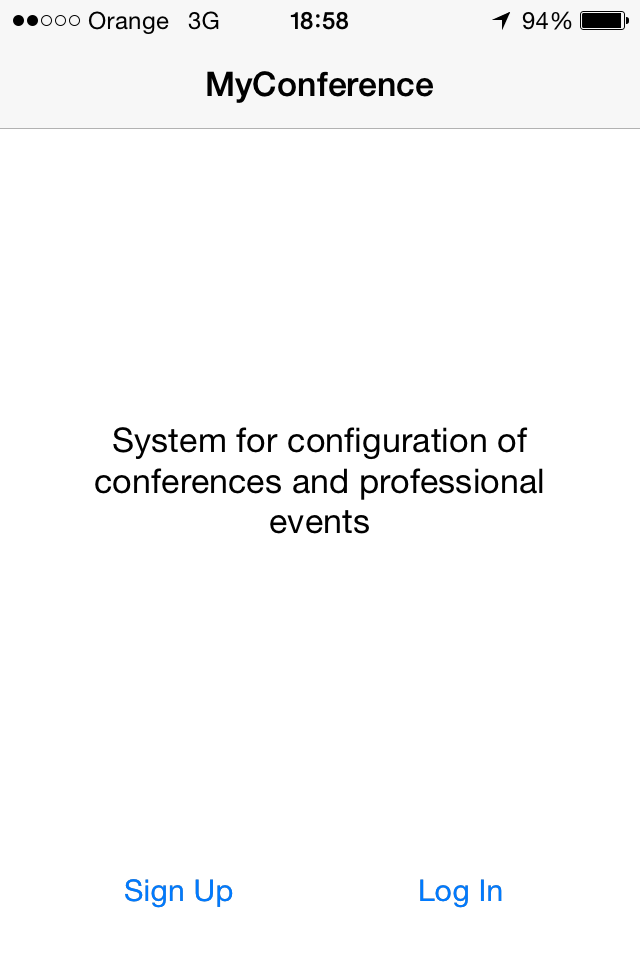
\includegraphics[width=0.42\textwidth]{./Imagenes/Bitmap/iOS/ios-main.png}}\\[20pt]
	   \hspace{0.1\linewidth}
	   %%----segunda subfigura----
	   \subfloat[]{
	        \label{fig:ios-signup}         %% Etiqueta para la segunda subfigura
	        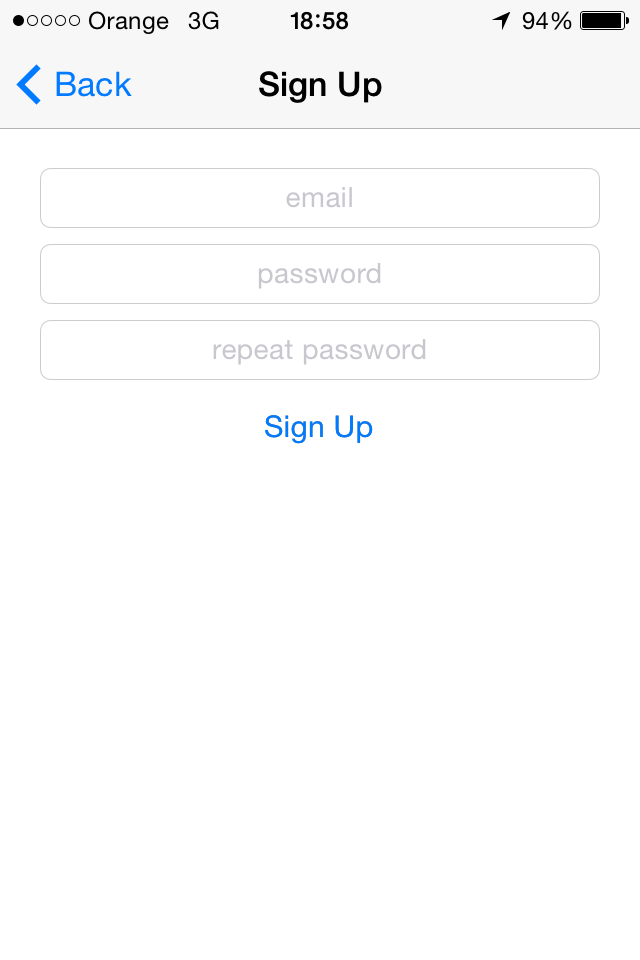
\includegraphics[width=0.42\textwidth]{./Imagenes/Bitmap/iOS/ios-signup.png}}
	   %%----tercera subfigura----
	   \subfloat[]{
	        \label{fig:ios-login}         %% Etiqueta para la tercera subfigura
	        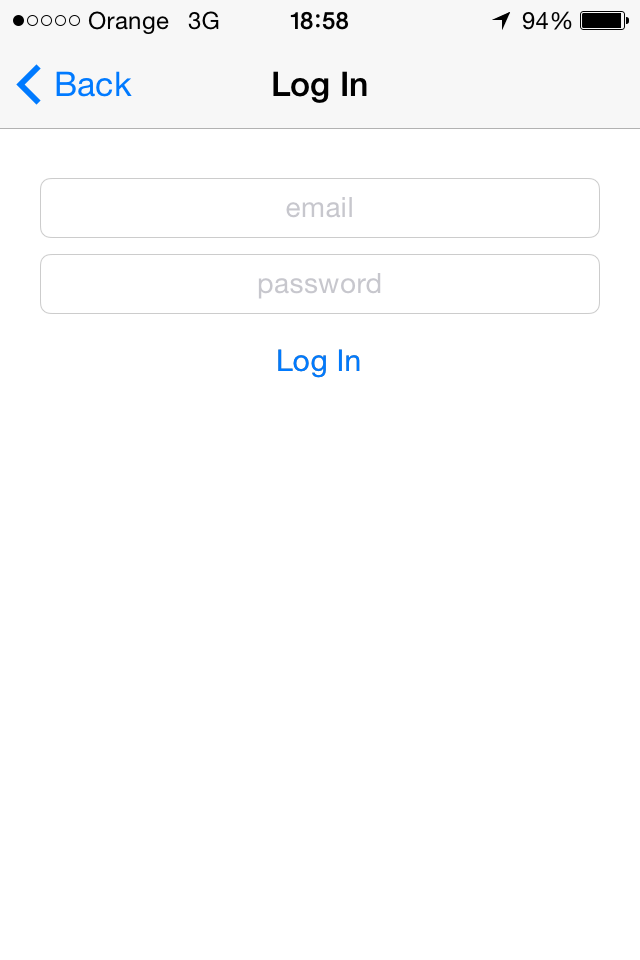
\includegraphics[width=0.42\textwidth]{./Imagenes/Bitmap/iOS/ios-login.png}}
	   \hspace{0.1\linewidth}
   \caption{Capturas de pantalla de la aplicaci�n iOS}
   \label{fig:ios-screenshots}                %% Etiqueta para la figura entera
\end{figure}

\subsection{Requisitos}

El software utilizado para el desarrollo de la aplicaci�n iOS es Xcode, un entorno de desarrollo utilizado para implementar aplicaciones tanto para iOS como para MacOS. Se puede descargar directamente desde el App Store y solo requiere tener creada una cuenta en iTunes para tener un Apple ID con el que registrar la descarga. 

\figura{Bitmap/iOS/xcode-logo}{width=0.3\textwidth}{fig:xcode-logo}%
    {Logo de Xcode.}

Xcode incluye todos los SDKs nativos de iOS necesarios para poder desarrollar la aplicaci�n. Tambi�n incluye simuladores para poder probar la aplicaci�n si no se dispone de un iPhone o un iPad. Hay simuladores para todos los tipos de iPhone y de iPad incluyendo todas las versiones disponibles del sistema iOS para cada tipo de dispositivo.

Es necesario disponer de un Mac ya que Xcode solo est� disponible para estos ordenadores. Tambi�n es recomendable disponer de un iPhone o un iPad para realizar las pruebas sobre dispositivos reales porque, aunque los simuladores proporcionados por Xcode funcionan bastante bien, son limitados con algunas caracter�sticas del sistema y no simulan al 100\% un dispositivo real.
